\documentclass[a4paper,10pt,portuguese]{article}
\usepackage[utf8]{inputenc}
\usepackage[portuguese]{babel}
\usepackage{ragged2e}
\usepackage{fancyvrb}
\usepackage{graphicx}

\title{Projeto do grupo 40 \\ Programação Orientada aos Objectos}
\author{Martins, José(a78821)\
        \and
        Costa, Mariana(a78824)\
        \and
        Quaresma, Miguel(a77049)
        }
\date{\today}

\begin{document}
 
\begin{titlepage}
\maketitle
\end{titlepage}
 
\tableofcontents
\newpage

\section{Introdução}
\textbf{UmER} é uma aplicação para transporte de passageiros e que permite que um utilizador realize viagens em táxis da UmER. Esta(aplicação) providencia mecanismos de criação de contas (de passageiros e motoristas), automóveis, realização de viagens e consulta das mesmas, alteração do estado dos motoristas(disponíveis ou indisponíveis). A aplicação permite ainda a permanência de dados aquando o fecho da mesma e a recuperação de um estado previamente guardado.
\newapge

\section{Arquitetura de Classes}

\begin{figure}[ht!]
    \centering
    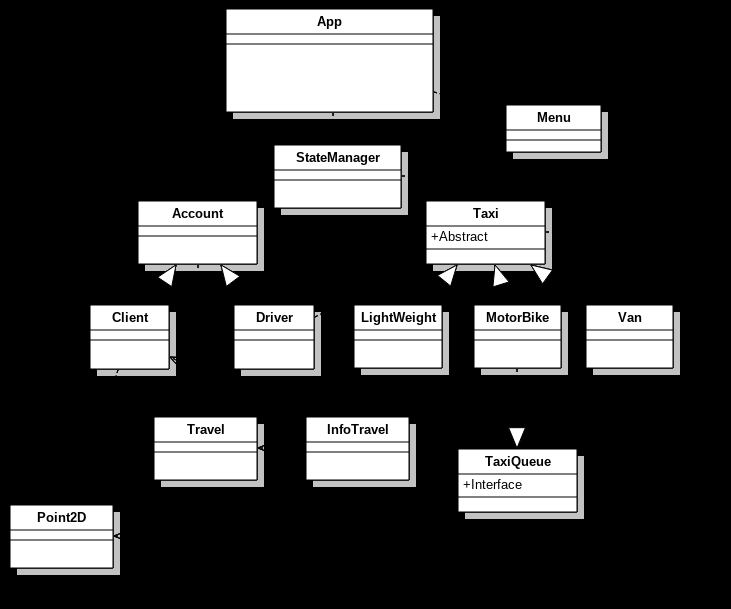
\includegraphics[width=120mm]{graph.jpg}
\end{figure}

\subsection{App}
A classe \texttt{App} corresponde à classe principal, sendo esta a classe que contém o método \texttt{Main} responsável por criar a instância da mesma(\texttt{App}).
Por forma a garantir que apenas é permitida uma instância da classe \texttt{App} é usado um contador que, após cada chamada ao construtor da classe, é, caso o seu valor seja 0, atualizado, incrementando-o em uma unidade. 
\begin{verbatim}
	if(App.count == 0){ 
        App.count=1;
        ...
    }else throw new TooManyInstancesException();
\end{verbatim}

Esta classe é responsável pela interação com o utilizador recorrendo para isso a três variáveis de instância: 
\begin{itemize}
\item[\texttt{StateManager}] :estado atual da aplicação(utilizadores, motoristas)
\item[\texttt{Menu}] :apresentação de menus de acordo com o utilizador
\item[\texttt{curUser}] :utilizador com sessão iniciada na aplicação no instante atual 
\end{itemize}

\subsection{StateManager}
A classe \texttt{StateManager} contém o estado atual da aplicação, em particular, os utilizadores registados, quer sejam \texttt{Client's} ou \texttt{Driver's}, estes são guardados numa variável de instância da classe \texttt{Map}, que faz a correspondência entre o email de cada utilizador e a classe \texttt{Account} correspondente.
A classe permite faculta ainda um conjunto de métodos para manipular a informação que guarda, permitindo a atualização da informação de um dado utilizador, a adição de novos utilizadores ou a verificação da existência de um dado utilizador com base num endereço de email.
\begin{verbatim}
public void addUser(Account nUser);
public boolean userExists(String uEmail);
public void updateUser(Account nInfo); 
\end{verbatim}
A criação de um utilizador apenas é permitida caso este ainda não esteja presente nos registos.

\subsection{Account}
A classe \texttt{Account} é a superclasse de duas outras, sendo elas as classes \texttt{Driver} e \texttt{Client}. Como tal, esta classe possui todos os componentes comuns às duas subclasses, sendo eles: \texttt{email}, \texttt{name}, \texttt{password}, \texttt{homeAdress}, \texttt{birthday} e as viagens realizadas(\texttt{travels}).
\subsubsection{Driver}
Sendo esta subclasse de \texttt{Account} herda tudo dessa classe, acrescentando o \texttt{status} do condutor(a trabalhar ou não), o \texttt{rating}, os kilómetros percorridos(\texttt{kmsTraveled}), a pontualidade(\texttt{punctuality}), e o taxi que o \texttt{Driver} usa(\texttt{car}).
\subsubsection{Client}
\subsection{Taxi}
\label{Taxi}
A classe \texttt{Taxi} é uma superclasse abstrata que guarda informações relativas aos veículos, nomeadamente a sua matrícula, a velocidade média, o preço cobrado por km, a localização atual do veículo e a fiablidade do mesmo. Esta última caraterística é gerada aleatoriamente cada vez que é requisitada uma viagem ao veículo, sendo depois usada como fator multiplicativo no cálculo do tempo real da viagem:
\begin{verbatim}
public double getEffectiveTime(double dist){
    this.genReliability();
    return dist/(this.averageSpeed*this.reliability);
}
    
// Randomly generates the reliability of a taxi before a ride
private void genReliability(){
    Random gen = new Random();
    this.reliability = gen.nextDouble()+0.01f;
}
\end{verbatim}
Esta classe possui três subclasses que diferem no tipo de táxi que representam, algo que influência se o táxi permite a existência de filas de espera ou não.
\begin{itemize}
	\item[\texttt{Motorbike\label{Motorbike}}]
	\item[\texttt{Van}]
	\item[\texttt{Lightweight}]
\end{itemize}
Os tipos de táxi que permitem fila de espera implementam a interface \texttt{TaxiQueue} que garante que determinadas operações de gestão das filas de espera se encontram disponíveis nas mesmas. Na implementação atual apenas a subclasse \texttt{Motorbike} permite filas de espera.
\subsection{Travel}
\subsection{InfoTravel}

\section{Aplicação e suas funcionalidades}

\section{Adição novos tipos de viaturas e motoristas na aplicação}
Como já foi referido, os diferentes tipos de viaturas são subclasses da classe abstrata Taxi(\ref{Taxi}), como tal, a elaboração de novos tipos de táxi requere apenas a criação de uma nova subclasse da classe Taxi e a implementação dos métodos requeridos pela classe abstrata bem como a implementação de métodos relevantes ao tipo de táxi em questão, por exemplo, um táxi do tipo TucTuc poderia suportar filas de espera visto se tratar de um tipo de veículo peculiar, como a mota(\ref{Motorbike}).
\newpage

\section{Conclusão}
Devio a alguns contratempos acabamos por nao implementar as companhias/empresas de taxis nem suas funções subjacentes(p.e. indicar o total faturado por uma viatura, ou empresa de táxis, num determinado período), porém com a atual estrutura do projeto é viável de se concretizar.

\end{document}
